\documentclass[a4paper]{article}

\usepackage[T1]{fontenc}
\usepackage[utf8]{inputenc}
\usepackage{lmodern}
\usepackage{amsmath}
\usepackage[a4paper, margin=1in]{geometry}
\usepackage{etoolbox}  
\usepackage{graphicx}
\usepackage{array} 
\usepackage{float}
\usepackage{caption}
\usepackage{booktabs}
\usepackage{tocloft}  % For better table of contents formatting

\patchcmd{\abstract}{\small}{\normalsize}{}{}
\patchcmd{\abstract}{\quotation}{}{}{}

\usepackage[english]{babel}
\usepackage{csquotes}

\usepackage[backend=biber]{biblatex} 
\bibliography{reference}

\begin{document}

\begin{titlepage}
    \begin{center}
        \vspace*{2cm} % Adjust vertical space as needed

        {\Huge \textbf{Carbon Intensity and Market Reaction: Evidence from Energy Sector Mergers and Acquisitions}}\\
        \vspace{2cm}
        {\LARGE Abdul Malik, Tejashree Vellanki, Sagrika Anand, Abhishek Phalke, Chiraag Katara}\\
        \vspace{1.5cm}
      
        \vfill

        \LARGE\textbf{Supervisor:}\\ Prof. Dr. Thorsten Martin\\
        \vspace{1cm}
        Submitted in partial fulfillment of the requirements for \\the course "Corporate Finance \& Valuation"\\
        \vspace{1cm}
        Frankfurt School of Finance \& Management\\
        March 2025
    \end{center}
\end{titlepage}

\section*{Meet the Team}

\begin{figure}[h]
    \centering
    \begin{minipage}{0.3\textwidth}
        \centering
        \includegraphics[width=0.9\textwidth]{Team/Picture1.jpg}
        \caption*{Abdul Malik\\8512905}
    \end{minipage}
    \hfill
    \begin{minipage}{0.3\textwidth}
        \centering
        \includegraphics[width=0.9\textwidth]{Team/Picture2.jpg}
        \caption*{Tejashree Vellanki\\8520289}
    \end{minipage}
    \hfill
    \begin{minipage}{0.3\textwidth}
        \centering
        \includegraphics[width=0.9\textwidth]{Team/Picture3.png}
        \caption*{Sagrika Anand\\8520107}
    \end{minipage}
    
    \vspace{0.5cm}
    \begin{minipage}{0.3\textwidth}
        \centering
        \includegraphics[width=0.9\textwidth]{Team/Picture4.JPG}
        \caption*{Abhishek Phalke\\8511026}
    \end{minipage}
    \hspace{0.5cm}
    \begin{minipage}{0.3\textwidth}
        \centering
        \includegraphics[width=0.9\textwidth]{Team/Picture5.jpg}
        \caption*{Chiraag Katara\\8520292}
    \end{minipage}
\end{figure}

\section*{Internal Distribution of Work}

\begin{table}[h]
    \centering
    \renewcommand{\arraystretch}{1.3}  % Increase the height of rows
    \begin{tabular}{|m{0.5\textwidth}|m{0.45\textwidth}|}
        \hline
        \textbf{Section} & \textbf{Author} \\
        \hline
        Research Question and Literature & Chiraag Katara \\
        \hline
        Hypothesis Development & Sagrika Anand \\
        \hline
        Empirical Design & Abdul Malik \\
        \hline
        Data and Descriptive Statistics & Abhishek Phalke \\
        \hline
        Results and Implications & Tejashree Vellanki \\
        \hline
        Introduction, Limitations and Future Research & Entire Team Effort \\
        \hline
        Python Programming and LaTeX & Abdul Malik \\
        \hline
        Data Origination and Cleanup & Abhishek Phalke and Tejashree Vellanki \\
        \hline
        Documentation and Discussions & Sagrika Ananad and Chiraag Katara \\
        \hline
    \end{tabular}
\end{table}
 
\newpage

\setcounter{tocdepth}{1}
\tableofcontents
\newpage
 
\begin{abstract}

This study examines the impact of carbon intensity on shareholder value in the context of mergers and acquisitions (M\&A) within the energy sector. Using an event study methodology, we analyze stock price reactions to acquisition deals where high-carbon-emitting ("Brown") firms acquire lower-emission (Green) targets. By leveraging data of the energy sector M\&A announcements from 2014 to 2024, we evaluate abnormal returns surrounding acquisition announcements to determine whether investors reward or penalize such strategic shifts toward sustainability.
\bigbreak
Our findings contribute to the ongoing debate on the financial viability of sustainability-driven corporate strategies. Preliminary evidence suggests that market reactions vary according to firm carbon intensity, deal structure, and broader industry trends. Although some investors may perceive "Green" acquisitions as a signal of long-term sustainability and innovation, others may remain skeptical due to concerns about green-washing or integration risks. This research provides insights for corporate decision-makers, investors, and policy makers navigating the intersection of environmental responsibility and financial performance in the energy sector.
\end{abstract}


\section{Introduction}
The global energy sector is experiencing a fundamental shift as companies navigate the challenges of climate change, technological advancements, and evolving regulatory landscapes. With annual renewable energy investments exceeding \$500 billion as of 2023, firms are increasingly integrating sustainability into their corporate strategies. Mergers and acquisitions (M\&As) have emerged as a key mechanism for energy companies to accelerate this transition, allowing them to reconfigure portfolios, achieve scale, and enhance financial stability in an environment of rising capital costs and market volatility.
\bigbreak
In recent years, \textbf{Green M\&As}—acquisitions of renewable energy and clean technology firms—have gained momentum, accounting for 35\% of the total energy sector M\&A deal value in 2023. However, the financial implications of such announcements remain a topic of debate. Do investors reward energy firms for pursuing Green acquisitions, or do they view these deals with skepticism? This question becomes particularly relevant when carbon-intensive ("Brown") firms acquire renewable assets. While such deals may signal a strategic shift toward sustainability, concerns over greenwashing, integration risks, and capital misallocation could negatively impact market perceptions.
\bigbreak
The existing literature offers mixed perspectives on this issue. Some studies suggest that ESG-driven strategies reduce capital costs and enhance long-term value creation (Giese \& Lee, 2020)\autocite{giese2020role}, while others highlight the challenges of integrating fundamentally different business models (Flammer, Toffel, \& Viswanathan, 2021)\autocite{flammer2021shareholder}. Additionally, investor reactions may vary depending on whether the acquiring firm has a history of sustainability commitments or is making an abrupt shift toward greener assets. Given these complexities, a deeper empirical investigation into the market's response to Green M\&As is warranted.
\bigbreak
This study aims to analyze the \textbf{short-term stock price impact} of Green M\&As in the energy sector, focusing on how market reactions differ based on the acquirer's environmental profile. Using an event study methodology with 3-day and 10-day event windows, we examine a sample of global energy sector M\&As from 2014 to 2024. Our findings will provide insights into whether Green acquisitions create or destroy short-term shareholder value and whether Brown firms experience a different market reaction compared to their greener counterparts.

 
\section{Research Question}

\textbf{``How do Green M\&As affect the stock prices of acquiring firms in the energy sector, and how does the market reaction differ based on the pre-existing environmental profile of the acquiring firm (Brown vs. Green)?"}
\bigbreak \noindent
This research is important for three key reasons:
\\
1. Investor Perceptions of Sustainability – The study explores whether investors reward firms for acquiring Green assets or remain skeptical, particularly when Brown firms make such acquisitions.
\\
2. Strategic Relevance – M\&A is a high-stakes corporate decision. Understanding the market's response to Green acquisitions can guide energy firms in optimizing their capital allocation strategies.
\\
3. Efficiency of Capital Allocation – If Green M\&As are systematically undervalued, it could discourage firms from making sustainability-driven investments, potentially slowing the global transition to cleaner energy systems.
\bigbreak \noindent
By addressing these questions, this study contributes to the ongoing discourse on sustainable finance, corporate strategy, and investor behavior in the energy transition.

\section{Literature Review}

\subsection{General Effects of M\&A on Stock Prices in the Energy Sector}
Mergers and acquisitions in the energy sector have been extensively studied, with research indicating that deal announcements typically trigger significant stock market reactions. (Jarrell \& Bradley, 1980) \autocite{jarrell1980} finds that target firms earn large positive abnormal returns, while acquirers often experience neutral or negative returns due to overpayment risks and integration challenges.

More recent studies provide more nuanced insights. (Andrade, Mitchell, and Stafford, 2001) \autocite{andrade2001} highlight that energy M\&A waves are driven by deregulation and consolidation, but market reactions depend on deal structure and financing methods. (Alexandridis, Antypas, and Travlos, 2016) \autocite{alexandridis2016} find that larger deals with higher synergies generate positive returns for both acquirers and targets. This suggests that, in the energy sector, economies of scale and regulatory synergies play a crucial role in determining M\&A success.

\subsection{Green M\&A and ESG Impact on Stock Prices}
M\&As involving corporate social responsibility (CSR)-driven assets, such as renewable energy acquisitions, have gained prominence due to the rise of ESG-focused investing. (Deng, Kang, \& Low, 2013) \autocite{deng2013} find that acquisitions by high-CSR firms generate stronger cumulative abnormal returns (CARs) than conventional deals, as they signal long-term sustainability commitments. Similarly, (Borghesi, Houston, \& Naranjo, 2014) \autocite{borghesi2014} show that acquiring environmentally aligned assets leads to positive stock reactions, particularly in regions with strict environmental regulations.

\subsection{Market Reaction When the Acquirer is a Polluting Firm ("Brown") Firm}
When Brown firms (e.g., fossil fuel companies) engage in Green M\&As, investor skepticism often arises. (Hong \& Kacperczyk, 2009) \autocite{hong2009} argue that firms in "sin" industries (e.g., oil and coal) face a valuation discount due to social norms, and CSR-driven acquisitions may be perceived as greenwashing unless backed by credible transition strategies.

However, (Amore \& Bennedsen, 2016) \autocite{amore2016} finds that while low-CSR acquirers often experience negative initial stock reactions, firms that communicate clear decarbonization plans eventually gain positive investor sentiment. This aligns with signaling theory, which suggests that Green M\&As could help Brown firms reduce their valuation discount, but only if they demonstrate real operational changes.

\subsection{Impact of ESG News on Firm Performance and Valuation}
(Derrien et al., 2024) \autocite{derrien2024} analyzes the relationship between negative ESG news and financial performance, finding that market reactions are driven by changes in revenue expectations rather than cost concerns. Their research is highly relevant for understanding market reactions to Green M\&As by Brown firms because:

\textbullet Investors may scrutinize Green M\&As for greenwashing if they doubt the acquirer's commitment to sustainability.

\textbullet The market primarily values ESG shifts based on expected revenue impact, meaning that if a Green M\&A does not clearly improve long-term cash flows, it may not create positive stock price reactions.

\subsection{Event Study Methodology in M\&A and ESG Research}
The event study methodology (MacKinlay, 1997) \autocite{mackinlay1997} is widely used to analyze stock price reactions to M\&A announcements. (Derrien et al., 2024)\autocite{derrien2024} emphasizes that ESG studies require event data, as ESG ratings are often slow-moving, whereas ESG news events trigger immediate market reactions.
\\
For this study, an event study methodology allows us to:

\textbullet Measure cumulative abnormal returns (CARs) around M\&A announcements.

\textbullet Differentiate between Green vs. non-Green acquisitions.

\textbullet Assess whether Brown firms experience different market reactions compared to Green acquirers.

\subsection{Identified Gaps}
The literature review highlights key gaps in understanding the stock price effects of Green M\&A in the energy sector:

\textbullet Limited empirical evidence on how Brown firms' Green acquisitions are perceived by the market.

\textbullet Conflicting views on investor reactions—some studies suggest positive signaling effects, while others highlight greenwashing risks.

\textbullet Lack of high-frequency event study analysis in this context, especially using recent data from 2014–2024.

This study addresses these gaps by empirically testing how investors react to Green M\&As and whether acquirer environmental profiles affect stock price movements.

\section{Hypothesis Development}
Based on the research question and the gaps in the existing literature, we develop the following hypotheses:
\bigbreak
\textbf{H1:} Energy sector M\&A announcements will, on average, be associated with positive abnormal returns for acquiring firms.
\smallbreak
Justification:
While M\&A announcements generally create value by generating synergies, prior research (King et al., 2004)\autocite{king2004} highlights that integration challenges often undermine shareholder gains. In the energy sector, mismatches between acquirers and targets (e.g., differences in business models) can influence abnormal returns.
\bigbreak
\textbf{H2:} Green M\&A announcements in the energy sector will be associated with higher positive abnormal returns for acquiring firms compared to non-Green M\&A announcements, but this effect will be contingent on investor perceptions of credibility, target quality, and integration feasibility.
\smallbreak
Justification:
Green acquisitions signal alignment with sustainability trends and may provide regulatory and financial benefits (Friede et al., 2015) \autocite{friede2015}. However, empirical evidence (Flammer et al., 2021) \autocite{flammer2021} suggests that markets react negatively to ESG acquisitions that lack operational substance, indicating that greenwashing concerns can mute expected returns. Furthermore, investor preferences may play a role—if shareholders of Brown firms prioritize dividends, Green acquisitions may be seen as capital misallocation (Friedman \& Heinle, 2016) \autocite{friedman2016disclosure}.

\bigbreak
\textbf{H3:} Green M\&A announcements by "Brown" acquiring firms will be associated with the highest positive abnormal returns, but only if the market perceives them as credible signals of strategic transformation and the acquisition target is financially strong.
\smallbreak
Justification:
Brown firms face an ESG discount (Hong \& Kacperczyk, 2009)\autocite{hong2009}, meaning a credible shift toward sustainability could reduce their perceived risk, leading to positive abnormal returns. However, some empirical evidence shows that the success of Brown-to-Green acquisitions depends on target credibility— large, profitable renewables generate positive stock reactions, whereas acquisitions of small or unproven companies can trigger skepticism. Integration risks and business model differences further complicate the valuation impact (King et al., 2004\autocite{king2004}.

\subsection{The Hypotheses as a Connection Between Research Question and Empirical Design}
The hypotheses serve as the critical link between our research question and empirical methodology by transforming theoretical expectations into testable predictions about market reactions to M\&A announcements. To empirically evaluate these hypotheses, we apply an event study methodology (MacKinlay, 1997)\autocite{mackinlay1997}, measuring abnormal stock returns around the announcement dates of global energy sector M\&A deals from 2014 to 2024. By comparing abnormal returns for Green versus non-Green M\&A announcements and differentiating based on the acquirer's environmental profile, we assess how sustainability considerations influence market valuations.

To further analyze Hypothesis 3, we employ a regression model examining the relationship between abnormal returns and the carbon intensity of acquiring firms, which serves as our primary metric for distinguishing Brown firms. This allows us to determine whether Brown acquirers experience stronger abnormal returns when engaging in Green M\&A.

By investigating these hypotheses, this study makes three key contributions:
\begin{itemize}
    \setlength{\itemsep}{0pt} 
    \item Extending the M\&A literature in the energy sector by providing an updated empirical analysis that captures the impact of the sector's ongoing transformation.
    \item Isolating the valuation effects of Green M\&As, offering evidence on whether and how sustainability considerations create value for acquiring firms.
    \item Providing insights into the transition strategies of carbon-intensive firms, assessing whether Green acquisitions meaningfully improve investor perceptions or merely generate short-term speculative gains.
\end{itemize}


\section{Empirical Design}

This study employs an event study methodology to examine the stock market reaction to merger and acquisition (M\&A) announcements in the energy sector. The primary objective is to estimate abnormal returns for acquiring firms relative to a market benchmark and to assess the impact of environmental performance, measured through carbon intensity, on these returns. Additionally, the analysis explores how the environmental orientation of target firms (Green vs. Brown) influences post-announcement market reactions.

To ensure robustness, the methodology accounts for potential confounding factors by carefully selecting event windows and applying robust statistical techniques to mitigate biases.

\subsection{Regression Specification}

To analyze the relationship between environmental factors and abnormal stock returns, the following regression model is estimated:

\begin{equation}
\label{eq:regression}
Abnormal\ Return_i = \alpha + \beta \cdot \log(Carbon\ Intensity_i + 1) + \varepsilon_i
\end{equation}

Where:
\begin{itemize}
    \setlength{\itemsep}{0pt} 
    \item \textbf{Abnormal Return\(_i\)} represents the benchmark-adjusted return for deal \(i\).
    \item \textbf{Carbon Intensity\(_i\)} is computed as the ratio of greenhouse gas (GHG) emissions in the preceeding year to annual revenue of the preceeding year for the acquiring firm.
    \item The \textbf{log transformation} of carbon intensity addresses skewness and extreme values.
    \item \(\beta\) captures the marginal impact of carbon intensity on deal performance.
    \item \(\varepsilon_i\) represents the error term.
\end{itemize}

\subsection{Analytical Subgroups}

The dataset is stratified into the following mutually exclusive groups for comparative analysis:

\begin{enumerate}
    \setlength{\itemsep}{0pt}
    \item \textbf{All Deals:} The full sample of qualifying M\&A announcements.
    \item \textbf{Green Target:} announcements where the target firm is classified as Green.
    \item \textbf{Brown Acquirer – Green Target:} A focused subset where Brown acquirers acquire Green targets.
\end{enumerate}

This subgroup classification allows for testing hypotheses related to investor response to environmentally motivated acquisitions and the strategic implications of acquiring Green firms.

\subsection{Identification Strategy and Preprocessing}

To enhance the reliability of findings, the following methodological refinements are implemented:
\begin{itemize}
    \setlength{\itemsep}{0pt}
    \item \textbf{Event Window Selection:} Abnormal returns are computed over \(\pm3\)-day and \(\pm10\)-day event windows surrounding the announcement date to capture both immediate and slightly delayed market responses.
    \item \textbf{Benchmark Selection:} Stock prices are benchmarked against the Energy Select Sector SPDR Fund (XLE) to control for broader energy market fluctuations.
    \item \textbf{Outlier Treatment:} Winsorization is applied at the 1st and 99th percentiles to mitigate the effects of extreme values stemming from speculative trading, rumors, or data anomalies.
    \item \textbf{Robustness Checks:} Additional robustness tests, including subsample analyses, volatility analyses and heteroskedasticity tests are conducted to validate the results. Based on Heteroskedasticity tests, robust standard errors are incorporated. heteroskedasticity results are available in \textbf{Table \ref{tab:heteroskedasticity_results3} and \ref{tab:heteroskedasticity_results10} in the Appendix} 
\end{itemize}

This methodology ensures a rigorous empirical design that systematically assesses the market impact of M\&A announcements while accounting for environmental factors.

\section{Data and Descriptive Statistics}

\subsection{Data Sources}

This study leverages multiple high-quality data sources:

\begin{itemize}
    \setlength{\itemsep}{0pt} 
    \item \textbf{M\&A announcements:} Sourced from Bloomberg, including deal metadata such as announcement dates, acquirer/target/seller names, ticker symbols, and deal values where available. The sample spans from January 2014 to December 2024, focusing on the energy and oil \& gas sectors.
    \item \textbf{GHG Emissions:} Acquirer-level emissions data were obtained from WRDS (via Trucost) and are reported in metric tons of CO$_2$ equivalent.
    \item \textbf{Revenue Data:} Acquirer revenues for the fiscal year preceding the deal were sourced from Bloomberg's equity section, reported in millions of USD.
    \item \textbf{Stock Prices:} Acquirer stock prices for \(\pm3\) and \(\pm10\) trading days around the deal announcement were retrieved using the Yahoo Finance API.
    \item \textbf{Benchmark Data:} XLE ETF prices were sourced from Bloomberg and used to benchmark acquirer returns, given its reliability, coverage, and alignment with the sectoral focus.
\end{itemize}

\subsection{Sample Selection Criteria}

The initial raw dataset consisted of 2,711 M\&A announcements. The following filters were applied to ensure data completeness and consistency:

\begin{itemize}
    \setlength{\itemsep}{0pt} 
    \item Inclusion was limited to publicly listed acquirers with available stock price data. 
    \item Acquirers were required to have both GHG emissions and revenue data for the fiscal year preceding the announcement.
\end{itemize}

After applying these selection criteria, the final dataset comprises 827 deals.

\subsection{Variable Construction and Integration}

The datasets were merged using acquirer ticker symbols and reference years. Key variable definitions include:

\begin{itemize}
    \setlength{\itemsep}{0pt} 
    \item \textbf{Carbon Intensity} was calculated as:
\begin{equation}
\label{eq:carbon_intensity}
Carbon\ Intensity = \frac{GHG\ Emissions}{Revenue}
\end{equation}
    This metric serves as an objective proxy for environmental performance.
    \item Stock prices were matched to announcement dates and used to compute percent returns over \(\pm3\) and \(\pm10\) days. 
    \item \textbf{Abnormal returns} were calculated by subtracting XLE benchmark returns for the same period from raw returns.
\end{itemize}

\subsection{Classification of Firms}

\begin{itemize}
    \setlength{\itemsep}{0pt} 
    \item \textbf{Acquirers:} Classified as Green if their carbon intensity fell in the bottom quartile (25\%), and Brown otherwise.
    \item \textbf{Targets:} Due to limited emissions or revenue data (as many targets are private or asset-based), classification was performed using keyword-based textual analysis of business descriptions. Firms were categorized as Green, Brown, or Neutral.
\end{itemize}

\subsection{Post-Processing and Standardization}

To ensure analytical readiness, the following steps were undertaken:

\begin{itemize}
    \setlength{\itemsep}{0pt} 
    \item Standardization of column names, units, and formats.
    \item Addressing missing values and inconsistencies.
    \item Exporting final datasets in structured CSV and JSON formats to support reproducibility and transparency in downstream modeling and visualization.
\end{itemize}

\subsection{Descriptive Statistics}
\textbf{Table \ref{tab:descriptive_stats} in the Appendix} of this paper presents summary statistics for cumulative abnormal returns (CAR) over both event windows (3-day and 10-day) across three different deal classifications:
\begin{enumerate}
\setlength{\itemsep}{0pt} 
\item Overall M\&A deals in the energy sector.
\item All firms acquiring Green targets.
\item Brown acquirers targeting Green firms.
\end{enumerate}

To maintain robustness in our study, we have employed below checks:
\begin{itemize}
\setlength{\itemsep}{0pt}
    \item  We have tested different event windows to study if the results hold consistent around the M\&A announcement dates or to understand if the announcement date has a bigger effect on value generation
    \item We used log transformation of carbon intensity to address skewness and normalize distribution
    \item We also removed extreme outliers to ensure that the results were not distorted and to make the findings of the research more generalizable
\end{itemize}

From the total sample of 827 M\&A deals, 23.1\% involve Green target acquisitions, while 16.6\% represent Brown firms acquiring Green targets. Across all cases, the mean CAR is positive, suggesting a generally favorable investor reaction. Notably, Brown acquirers targeting Green firms exhibit the highest positive returns (+0.811\% in the [-3,+3] window and +0.783\% in the [-10,+10] window). However, none of these CARs are statistically significant, indicating that the observed effects could be driven by randomness.

The graphs and figure showing data distribution and mean abnormal returns across different classifications are available as \textbf{Figure \ref{fig:dealdist}, Figure \ref{fig:3day_MAR}, Figure \ref{fig:10day_MAR}, Figure \ref{fig:3day_WMAR}, Figure \ref{fig:10day_WMAR},  in the Appendix.} 

The weighted returns for any firm acquiring Green targets and Brown firms acquiring Green targets are positive, suggesting that larger M\&A deals tend to generate better market performance. Interestingly, Brown firms acquiring Green targets achieve higher weighted returns (+0.814\% in the 3-day window and +2.245\% in the 10-day window) compared to Green firms acquiring Green targets. This finding suggests that investors reward Brown firms transitioning towards sustainability more than Green firms acquiring similar companies.

In terms of volatility, the standard deviation is highest in the overall sample (9.87\%), slightly lower in Green target acquisitions (9.84\%), and further reduced in Brown-on-Green deals (9.32\%). This suggests that market reactions to Green acquisitions are relatively stable and that price volatility increases over longer periods. It also implies that Green acquisitions are perceived as less risky compared to broader M\&A announcements in the energy sector.

Additionally, a negative correlation between Carbon Intensity and CAR among Brown acquirers suggests that firms with lower carbon emissions receive stronger positive market reactions.

\section{Results}
The histograms and scatterplot figures showing event study and regression results across different classifications are available in \textbf{ Appendix as }:
\begin{itemize}
\item3 day event window : \\
\textbf{Figure \ref{fig:3_WinMAR}, Figure \ref{fig:3day_AWARD}, Figure \ref{fig:3day_ACIAR}, Figure \ref{fig:3day_GWARD}, Figure \ref{fig:3day_GCIAR}, Figure \ref{fig:3day_BWARD}, Figure \ref{fig:3day_BCIAR} }
\item 10 day event window: \\
\textbf{ Figure \ref{fig:10_WinMAR}, Figure \ref{fig:10day_AWARD}, Figure \ref{fig:10day_ACIAR}, Figure \ref{fig:10day_GWARD}, Figure \ref{fig:10day_GCIAR}, Figure \ref{fig:10day_BWARD}, Figure \ref{fig:10day_BCIAR}}
\end{itemize}

\subsection{Event Study Analysis}
To assess the impact of M\&A announcements on stock prices, we conduct an event study examining cumulative abnormal returns (CAR) over both short-term (-3, +3) and slightly longer-term (-10, +10) windows around announcement date.

\subsubsection{Three-Day Event Window [-3,+3]}
Our findings indicate a negative relationship between carbon intensity and abnormal returns. Specifically, for Brown acquirers acquiring Green targets, we find a statistically significant coefficient of -0.617 with a p-value of 0.039. This suggests that the market reacts favorably when Brown firms with lower carbon intensity acquire Green targets, potentially due to perceptions of sustainability-driven strategic value, regulatory advantages, or improved ESG credentials.

The results for our sample in the 3-day event window are provided in Table \textbf{\ref{tab:3_Day_results} in the Appendix.} 

\subsubsection{Ten-Day Event Window [-10,+10]}
Extending the analysis to a longer window, we observe a similar negative effect (-0.632), though it is statistically weaker (p = 0.16). This suggests that while short-term market reactions are significant, long-term impact may be influenced by other factors such as strategic synergies, macroeconomic conditions, and investor reassessment of deal prospects.

The results for our sample in the 10-day event window are provided in Table \textbf{\ref{tab:10_Day_results} in the Appendix.} 

\subsection{Regression Analysis}
To further explore the relationship between carbon intensity and M\&A returns, we run a regression analysis using log-transformed carbon intensity as the independent variable and cumulative abnormal returns (CAR) as the dependent variable.

\begin{equation}
\label{eq:car_regression}
    CAR_{i} = \beta \cdot \text{Carbon Intensity}_{i} + \epsilon_{i}
\end{equation}

Our results indicate that carbon intensity has a negative and statistically significant effect on abnormal returns in the short-term event window, confirming that markets penalize high-carbon acquirers in Green M\&A announcements. However, the relatively low R-squared values (0.031 for short-term CAR and 0.0146 for long-term CAR) suggest that carbon intensity alone does not fully explain abnormal returns. Other financial, strategic, and macroeconomic variables likely play a role in shaping investor sentiment.

Furthermore, our weighted returns analysis shows that larger and higher-valued deals exhibit stronger positive abnormal returns, particularly when Brown firms acquire Green targets. This reinforces the idea that investors may view such deals as an effective transition strategy towards sustainability.

\subsection{Revisiting the Value Implications of Brown-to-Green Acquisitions}
The conventional view suggests that Brown firms acquiring Green targets should destroy value due to potential integration challenges, cultural mismatches, and investor skepticism regarding greenwashing. However, our results indicate otherwise: Brown acquirers targeting Green firms experience positive abnormal returns (+0.75\%), higher than Brown-Brown acquisitions (-0.64\%).

\subsubsection{Carbon Intensity and Market Response}
A deeper analysis reveals that the market reaction to Brown-Green acquisitions is not uniform but conditional on the acquirer's carbon intensity. Specifically:
\begin{itemize}
    \item The \textbf{lowest-carbon Brown firms} generate \textbf{+3.09\%} returns when acquiring Green targets.
    \item The \textbf{highest-carbon Brown firms}, however, experience negative abnormal returns of \textbf{-0.48\%}.
\end{itemize}
This suggests that investors reward Brown firms with credible environmental transitions while penalizing those perceived as engaging in greenwashing.

\subsubsection{Deal Size as a Moderating Factor}
Our findings also indicate that the \textbf{size of the deal} influences market reactions:
\begin{itemize}
    \item \textbf{Small deals} generate the highest returns (+2.55\%).
    \item \textbf{Very large deals}, in contrast, exhibit negative abnormal returns (-0.34\%).
\end{itemize}
This contradicts suggesting that large deals should generate more value. One possible explanation is that our sample excludes firms that do not report greenhouse gas (GHG) emissions, introducing a bias toward more transparent firms. Since GHG disclosure often correlates with stronger environmental management, this subset of firms may be perceived as more capable of successfully integrating Green targets.

\subsubsection{Reconciling the Conflicting Evidence}
The apparent contradiction—why some Brown-to-Green acquisitions create value while others do not—can be resolved by considering \textbf{three key factors}:
\begin{enumerate}
    \item \textbf{Acquirer's Carbon Profile} – Lower-carbon Brown firms are rewarded, while high-carbon firms are penalized.
    \item \textbf{Deal Size} – Smaller deals yield higher returns, potentially due to easier integration.
    \item \textbf{Transparency Bias} – Firms in our sample are likely more environmentally responsible than those in prior studies, affecting comparability.
\end{enumerate}

These findings suggest that \textbf{it is not simply the act of acquiring a Green firm that determines value creation but rather the acquirer's existing environmental credibility and the scale of the acquisition}.Investors appear to differentiate between Brown firms genuinely transitioning toward sustainability and those attempting to signal Green commitment without substantive change.

\subsection{Discussion}
Overall, our results suggest that investor sentiment towards Green M\&A is nuanced. While markets favor Brown firms making strategic Green acquisitions, high carbon intensity remains a negative factor in market reactions. These findings contribute to the growing discourse on ESG-driven M\&A, highlighting both the opportunities and challenges faced by transitioning firms in the energy sector.

\section{Limitations and Future Research}
While our findings provide valuable insights into the market reaction to Brown-Green M\&A announcements, several limitations should be acknowledged:

\begin{itemize}
    \item \textbf{Sample Composition Bias} – Our dataset includes firms that report greenhouse gas (GHG) emissions, potentially introducing a selection bias. Firms that do not disclose emissions may exhibit different M\&A behavior, limiting the generalizability of our results. Future research should explore how undisclosed emissions influence market reactions.
    
    \item \textbf{Causality and Unobserved Factors} – The observed market response to M\&A deals could be driven by factors beyond carbon intensity, such as synergies, corporate governance, or macroeconomic conditions. A causal inference approach (e.g., instrumental variable estimation) could strengthen the robustness of our findings.

    \item \textbf{Investor Perceptions and ESG Ratings} – This study assumes that investors interpret Brown-to-Green acquisitions as a signal of sustainability commitment. However, investor sentiment may vary depending on ESG rating agencies, regulatory environments, or industry-specific factors. A deeper analysis incorporating qualitative investor sentiment data could offer further insights.

    \item \textbf{Long-Term Performance} – Our event study focuses on short-term abnormal returns, which may not fully capture the long-term strategic benefits or risks associated with Green acquisitions. Future research could examine post-merger financial performance and carbon reduction progress to assess whether these acquisitions create sustainable value.
\end{itemize}

\section{Conclusion}
This study examines the market reaction to M\&A announcements in the energy sector, with a particular focus on Brown acquirers targeting Green firms. Our findings show that M\&A deals in Energy Industry have mixed returns. More specifically, we show that investor response depends critically on the \textbf{carbon profile of the acquirer and the size of the deal}:

\begin{itemize}
    \item \textbf{Lower-carbon Brown firms} experience \textbf{positive abnormal returns} when acquiring Green targets, suggesting that investors reward credible sustainability transitions.
    
    \item \textbf{High-carbon Brown firms}, on the other hand, experience negative abnormal returns, indicating skepticism regarding potential greenwashing.
    
    \item \textbf{Smaller deals} yield higher market reactions, while very large deals tend to dilute perceived value.
\end{itemize}

These findings highlight the complexity of sustainability-driven M\&A. Investors differentiate between \textbf{genuine strategic transitions} and \textbf{symbolic environmental commitments}, underscoring the importance of credibility in corporate sustainability strategies. Future research should explore how post-merger environmental performance influences long-term firm valuation, regulatory responses, and stakeholder engagement.

\printbibliography

\newpage
\appendix
\section{Appendix}

\subsection{Tables}

\begin{table}[htbp]
\centering
\small
\renewcommand{\arraystretch}{1.3} 
\caption{Summary Statistics of Cumulative Abnormal Returns (CAR)}
\label{tab:descriptive_stats}
\resizebox{\textwidth}{!}{
\scriptsize
\begin{tabular}{|c|c|c|c|c|>{\centering\arraybackslash}p{2.5cm}|} 
\hline
\textbf{Variable} & \textbf{Obs.} & \textbf{Mean} & \textbf{Median} & \textbf{SD} & \textbf{ Weighted Return}\\
\hline
\multicolumn{6}{|l|}{\textbf{Panel A: All Deals}} \\
\hline
CAR (3 Days) & 827 & 0.097\% & 0.067\% & 6.690\% & -0.610\% \\
CAR (10 Days) & 827 & 0.342\% & 0.193\% & 9.870\% & -0.434\% \\
\hline
\multicolumn{6}{|l|}{\textbf{Panel B: All Firms Acquiring Green Targets}} \\
\hline
CAR (3 Days) & 191 & 0.726\% & 0.252\% & 6.100\% & 0.547\% \\
CAR (10 Days) & 191 & 0.581\% & 0.231\% & 9.840\% & 1.391\% \\
\hline
\multicolumn{6}{|l|}{\textbf{Panel C: Brown Acquiring Green}} \\
\hline
CAR (3 Days) & 137 & 0.811\% & 0.088\% & 6.250\% & 0.814\% \\
CAR (10 Days) & 137 & 0.783\% & 0.954\% & 9.320\% & 2.245\% \\
\hline
\end{tabular}
}
\end{table} 

 
\begin{table}[htbp]
    \centering
    \caption*{Event Study Results}
    \begin{minipage}{0.48\textwidth}
        \centering
        \caption{for [-3,+3] Event Window}
        \label{tab:3_Day_results}
        \begin{tabular}{lcc}
            \hline
            & CAR [-3,+3] & p-value \\
            \hline
            Carbon Intensity & -0.617 & 0.039 \\
            R-squared & 0.031 & \\
            Observations & 827 & \\
            \hline
        \end{tabular}
    \end{minipage}
    \hfill
    \begin{minipage}{0.48\textwidth}
        \centering
        \caption{for [-10,+10] Event Window}
        \label{tab:10_Day_results}
        \begin{tabular}{lcc}
            \hline
            & CAR [-10,+10] & p-value \\
            \hline
            Carbon Intensity & -0.632 & 0.16 \\
            R-squared & 0.0146 & \\
            Observations & 827 & \\
            \hline
        \end{tabular}
    \end{minipage}
\end{table}

\begin{table}[htbp]
    \centering
    \caption{Heteroskedasticity Test Results for 3 day Event Window}
    \label{tab:heteroskedasticity_results3}
    \begin{tabular}{lccc}
        \hline
        \textbf{Test} & \textbf{Test Statistic} & \textbf{P-value} \\
        \hline
        Breusch-Pagan Test & 42.857 & 0.000*** \\
        White Test & 51.234 & 0.000*** \\
        Goldfeld-Quandt Test & 2.345 & 0.012** \\
        \hline
        \multicolumn{3}{p{0.8\textwidth}}{\textit{Notes:} Significance levels: * p<0.1; ** p<0.05; *** p<0.01.} \\
        \multicolumn{3}{p{0.8\textwidth}}{Heteroskedasticity observed therefore robust standard errors included in analysis.} \\
    \end{tabular}
    \bigbreak \bigbreak
    \caption{Heteroskedasticity Test Results for 10 day Event Window}
    \label{tab:heteroskedasticity_results10}
    \begin{tabular}{lccc}
        \hline
        \textbf{Test} & \textbf{Test Statistic} & \textbf{P-value} \\
        \hline
        Breusch-Pagan Test & 7.596 & 0.006*** \\
        White Test & 8.292 & 0.016** \\
        \hline
        \multicolumn{3}{p{0.8\textwidth}}{\textit{Notes:} Significance levels: * p<0.1; ** p<0.05; *** p<0.01.} \\
        \multicolumn{3}{p{0.8\textwidth}}{Heteroskedasticity observed therefore robust standard errors included in analysis.} \\
    \end{tabular}
\end{table}


\newpage
\subsection{Figures}

\begin{figure}[htbp]
    \centering
    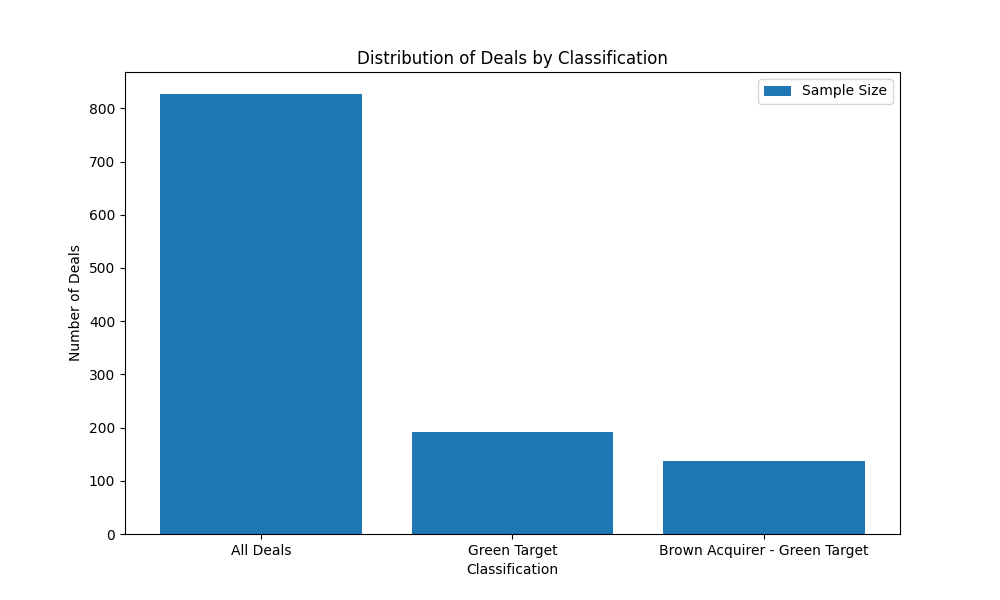
\includegraphics[width=0.8\textwidth]{figures/alldeals.png}
    \caption{Distribution of Deals by Classification}
    \label{fig:dealdist}
\end{figure}

\begin{figure}[htbp]
\centering
    \begin{minipage}{0.48\textwidth}
        \centering
        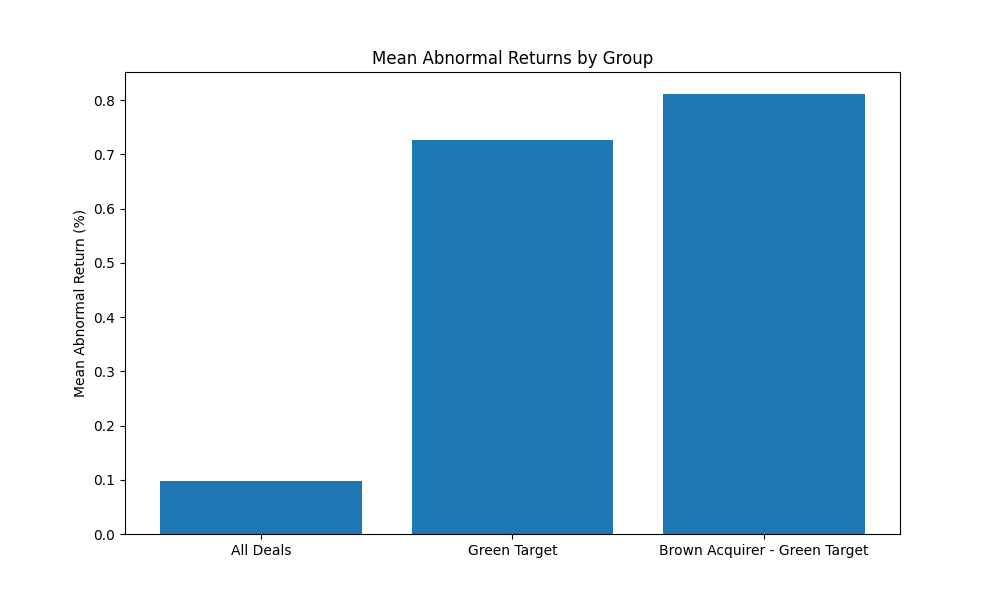
\includegraphics[width=\textwidth]{figures/mean_abnormal return 3 day.png}
        \caption{Mean Abnormal Return (3-Day)}
        \label{fig:3day_MAR}
    \end{minipage}
    \hfill
    \begin{minipage}{0.48\textwidth}
        \centering
        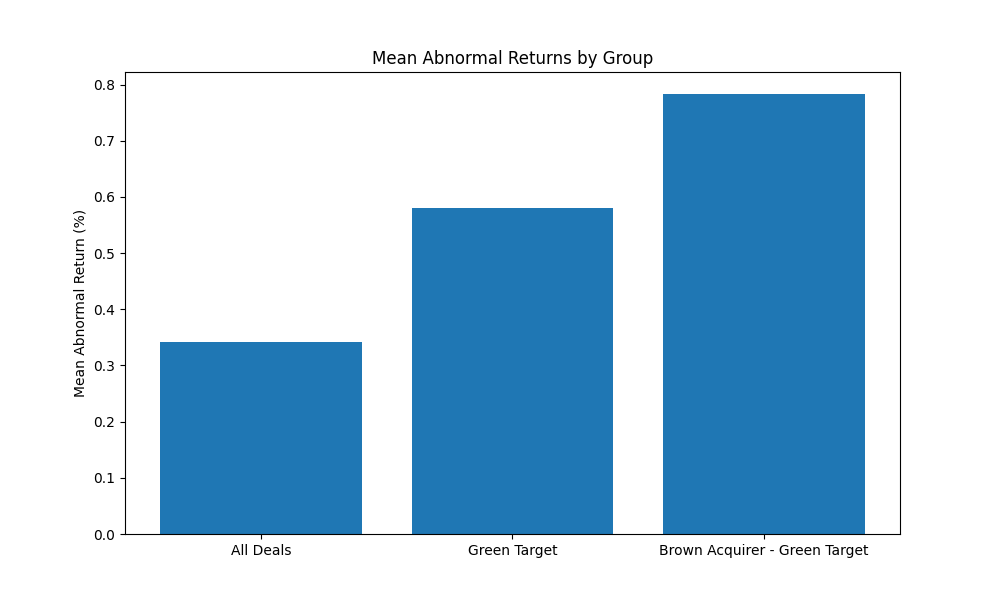
\includegraphics[width=\textwidth]{figures/mean_abnormal return 10 day.png}
        \caption{Mean Abnormal Return (10-Day)}
        \label{fig:10day_MAR}
    \end{minipage}
\end{figure}

\begin{figure}[htbp]
   \begin{minipage}{0.48\textwidth}
        \centering
        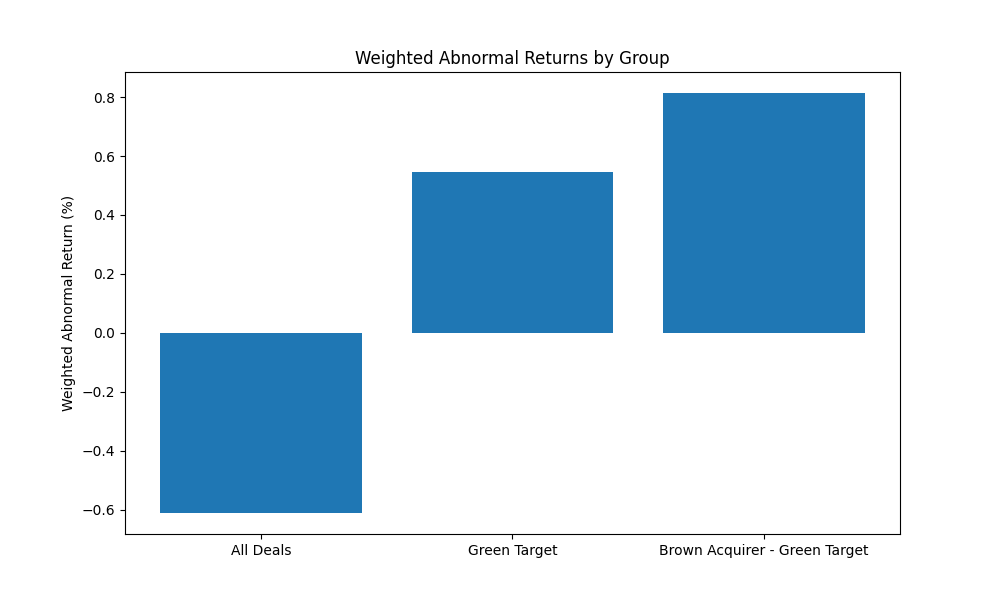
\includegraphics[width=\textwidth]{figures/mean_abnormal weighted return 3 day.png}
        \caption{Weighted Mean Abnormal Return (3-Day)}
        \label{fig:3day_WMAR}
    \end{minipage}
    \hfill
    \begin{minipage}{0.48\textwidth}
        \centering
        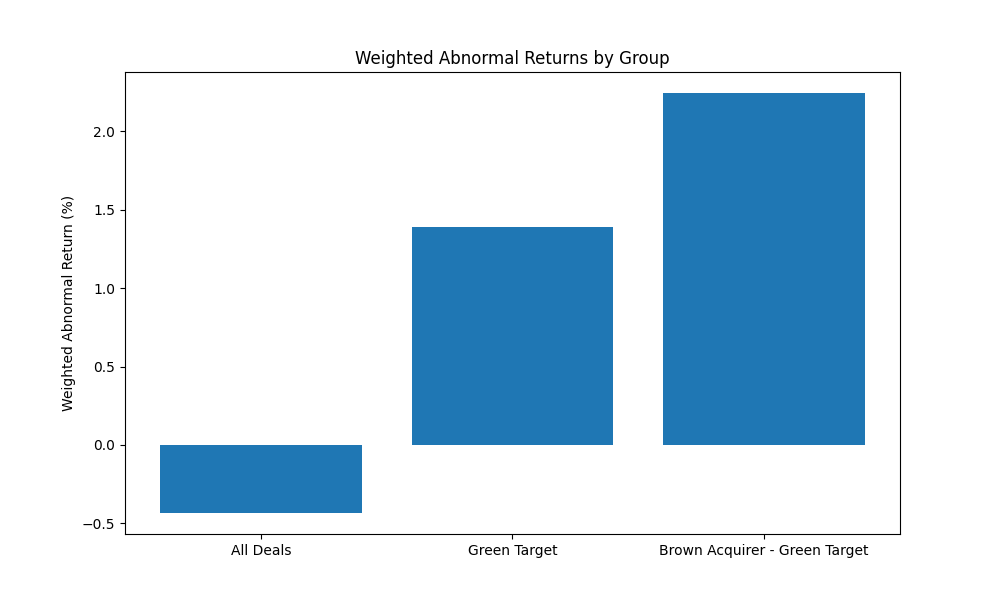
\includegraphics[width=\textwidth]{figures/mean_abnormal weighted return 10 day.png}
        \caption{Weighted Mean Abnormal Return (10-Day)}
        \label{fig:10day_WMAR}
    \end{minipage}
\end{figure}

\begin{figure}[htbp]
    \centering
    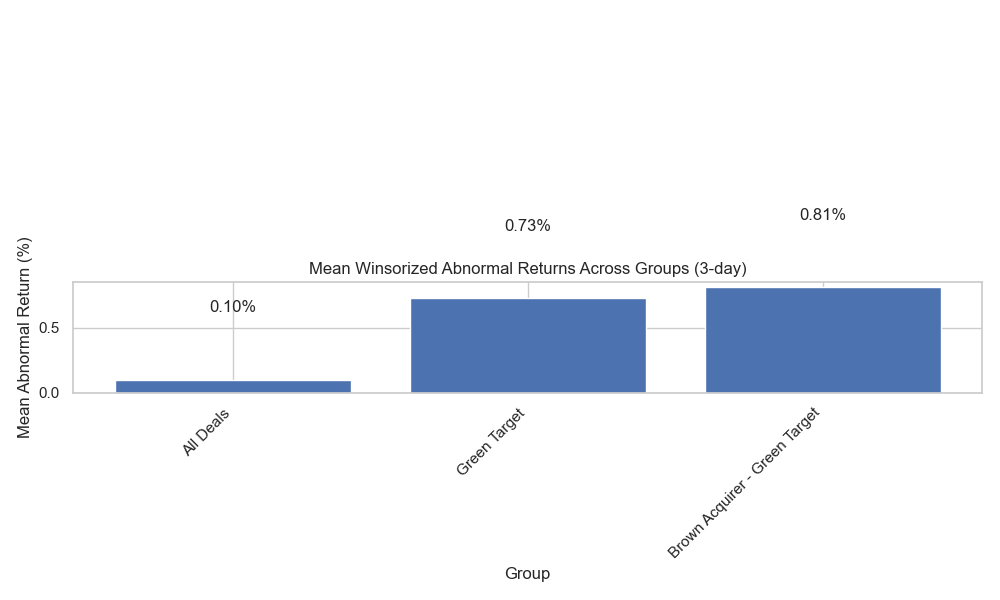
\includegraphics[width=0.8\textwidth]{visualizations/mean_abnormal_returns_comparison_3day.png}
    \caption{3 day Winsorised Mean Ab. Return }
    \label{fig:3_WinMAR}
\end{figure}

\begin{figure}[htbp]
\caption*{All Deals 3 Day Results}
   \begin{minipage}{0.48\textwidth}
        \centering
        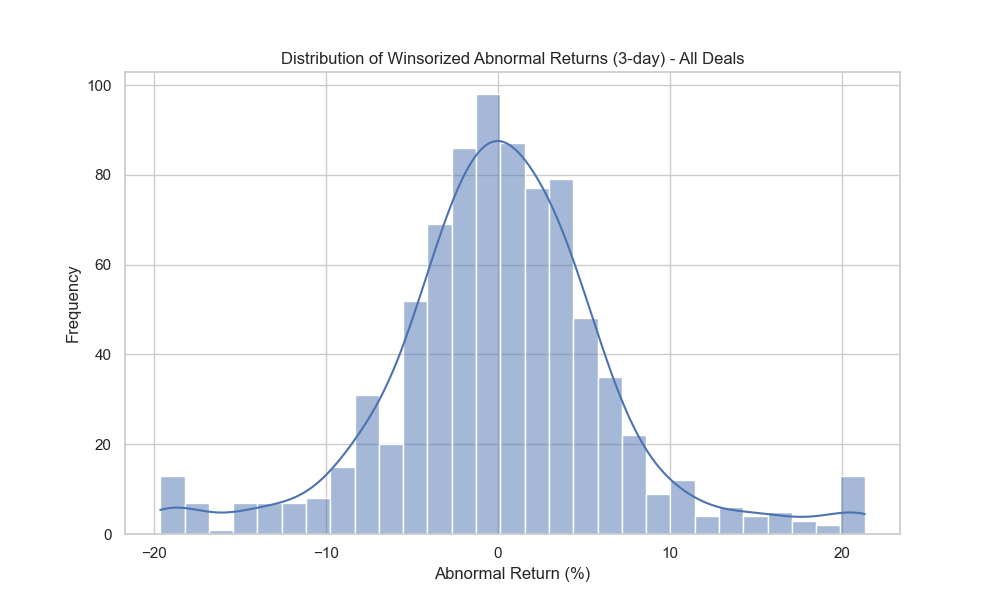
\includegraphics[width=\textwidth]{visualizations/all_deals_3day_ar_distribution.png}
        \caption{Abnormal Return Distribution}
        \label{fig:3day_AWARD}
    \end{minipage}
    \hfill
    \begin{minipage}{0.48\textwidth}
        \centering
        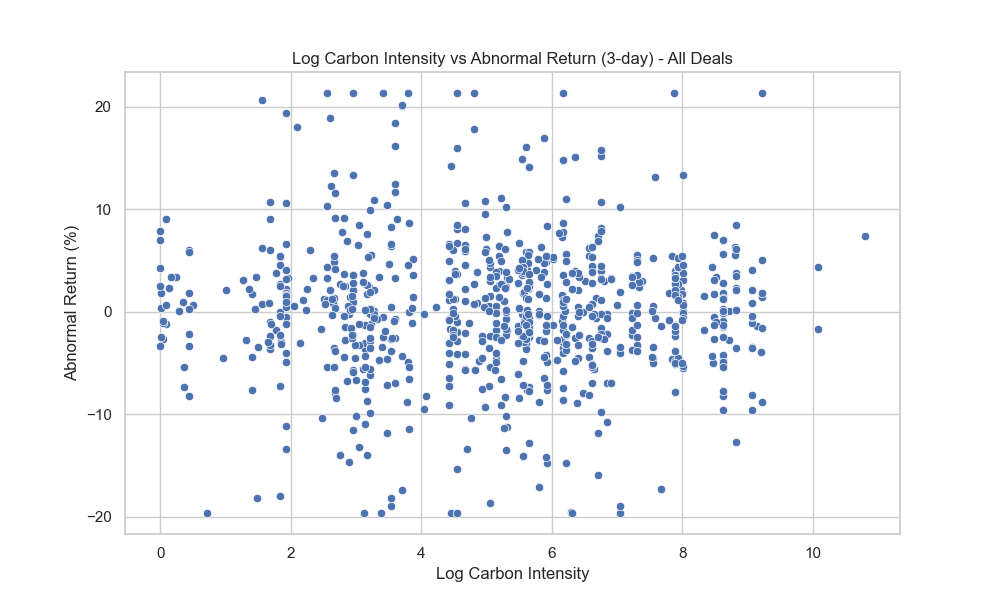
\includegraphics[width=\textwidth]{visualizations/all_deals_3day_carbon_vs_ar.png}
        \caption{Log CI Vs AR regression}
        \label{fig:3day_ACIAR}
    \end{minipage}
\end{figure}

\begin{figure}[htbp]
\caption*{Any Acquirer - Green Targets 3 Day Results}
   \begin{minipage}{0.48\textwidth}
        \centering
        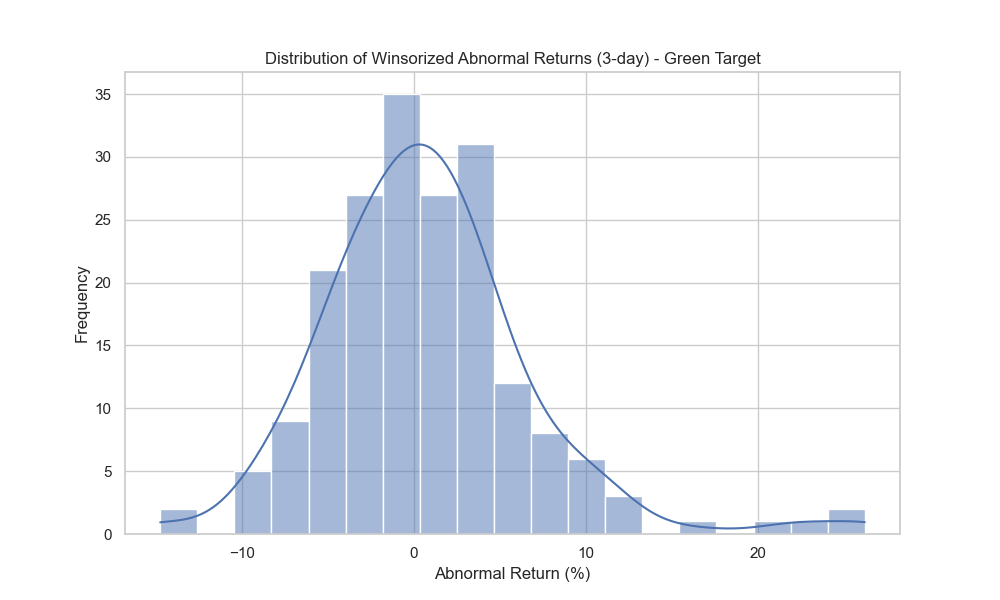
\includegraphics[width=\textwidth]{visualizations/green_target_3day_ar_distribution.png}
        \caption{Abnormal Return Distribution}
        \label{fig:3day_GWARD}
    \end{minipage}
    \hfill
    \begin{minipage}{0.48\textwidth}
        \centering
        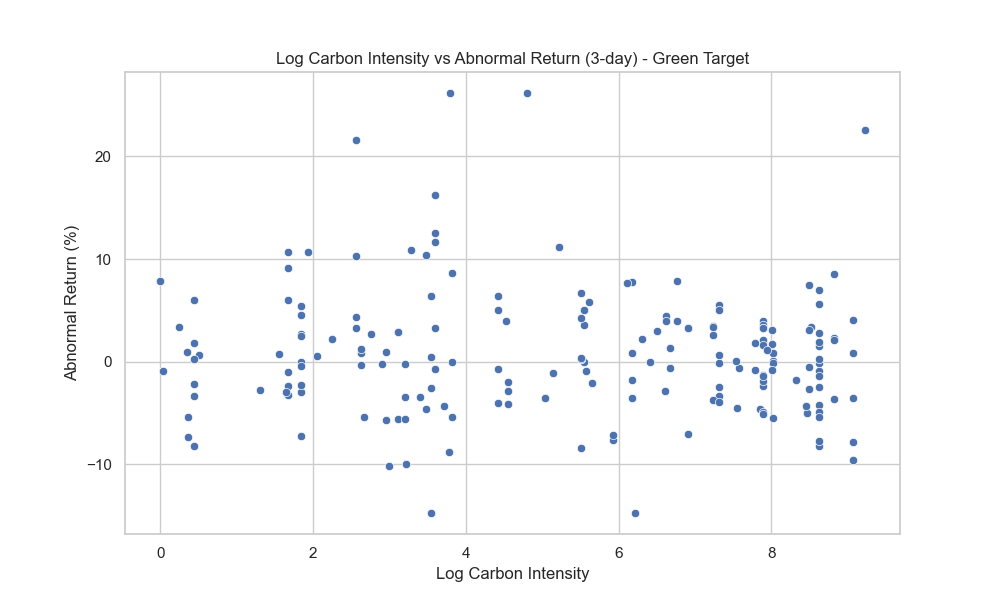
\includegraphics[width=\textwidth]{visualizations/green_target_3day_carbon_vs_ar.png}
        \caption{Log CI Vs AR regression}
        \label{fig:3day_GCIAR}
    \end{minipage}
\end{figure}

\begin{figure}[htbp]
\caption*{Brown Acquirer - Green Targets 3 Day Results}
   \begin{minipage}{0.48\textwidth}
        \centering
        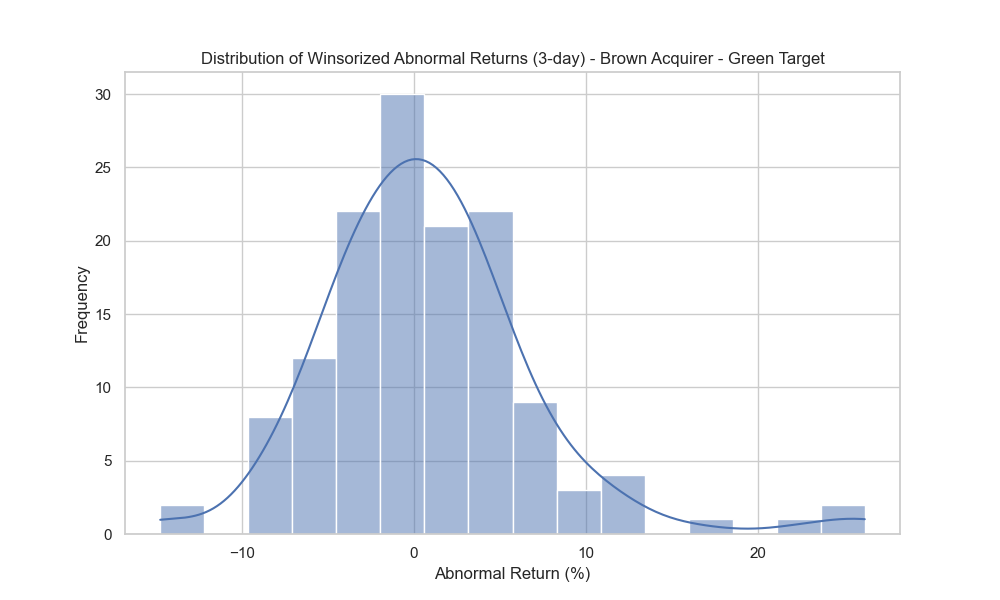
\includegraphics[width=\textwidth]{visualizations/brown_acquirer_-_green_target_3day_ar_distribution.png}
        \caption{Abnormal Return Distribution}
        \label{fig:3day_BWARD}
    \end{minipage}
    \hfill
    \begin{minipage}{0.48\textwidth}
        \centering
        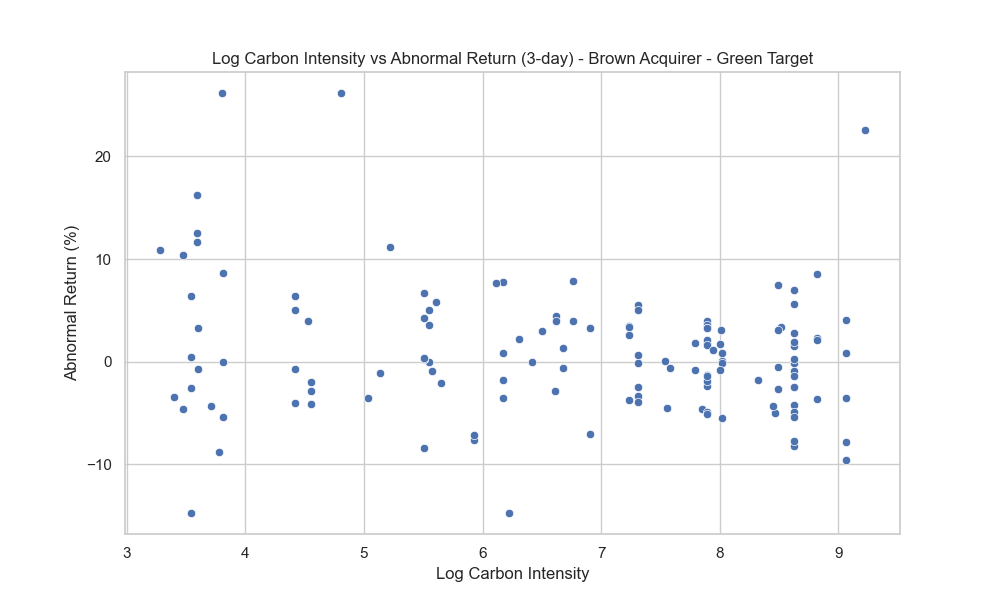
\includegraphics[width=\textwidth]{visualizations/brown_acquirer_-_green_target_3day_carbon_vs_ar.png}
        \caption{Log CI Vs AR regression}
        \label{fig:3day_BCIAR}
    \end{minipage}
\end{figure}

\begin{figure}[htbp]
    \centering
    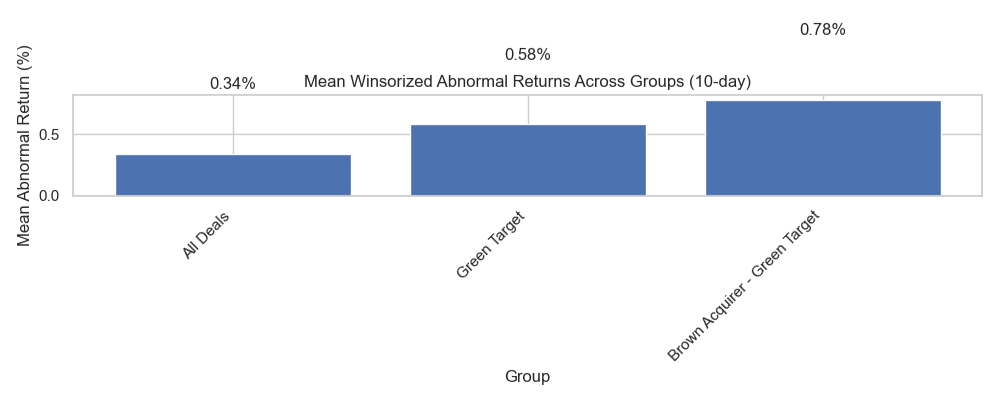
\includegraphics[width=0.8\textwidth]{visualizations1/mean_abnormal_returns_comparison_10day.png}
    \caption{10 day Winsorised Mean Ab. Return }
    \label{fig:10_WinMAR}
\end{figure}
 

\begin{figure}[htbp]
\caption*{All Deals 10 Day Results}
   \begin{minipage}{0.48\textwidth}
        \centering
        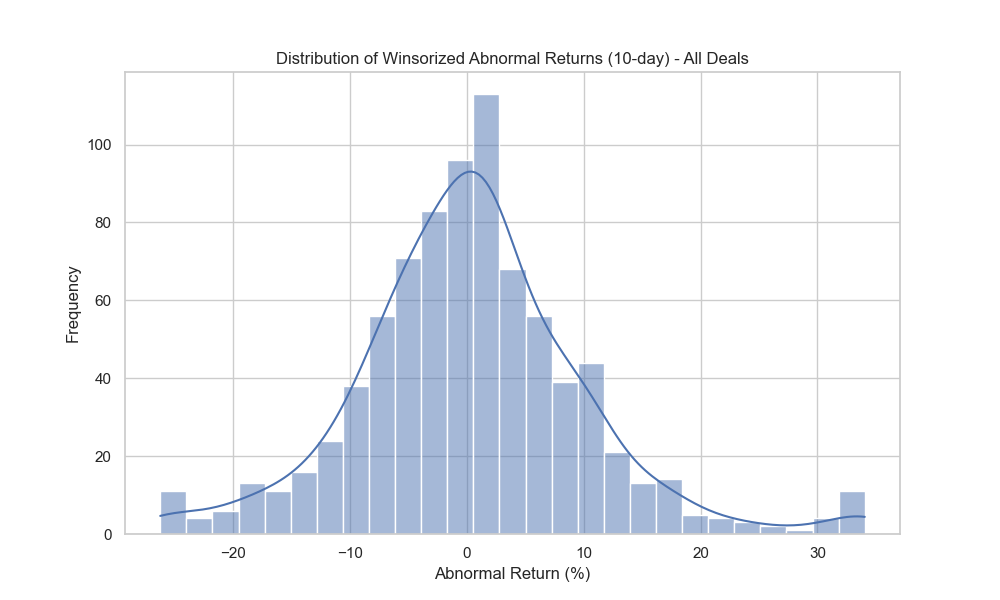
\includegraphics[width=\textwidth]{visualizations1/all_deals_10day_ar_distribution.png}
        \caption{Abnormal Return Distribution}
        \label{fig:10day_AWARD}
    \end{minipage}
    \hfill
    \begin{minipage}{0.48\textwidth}
        \centering
        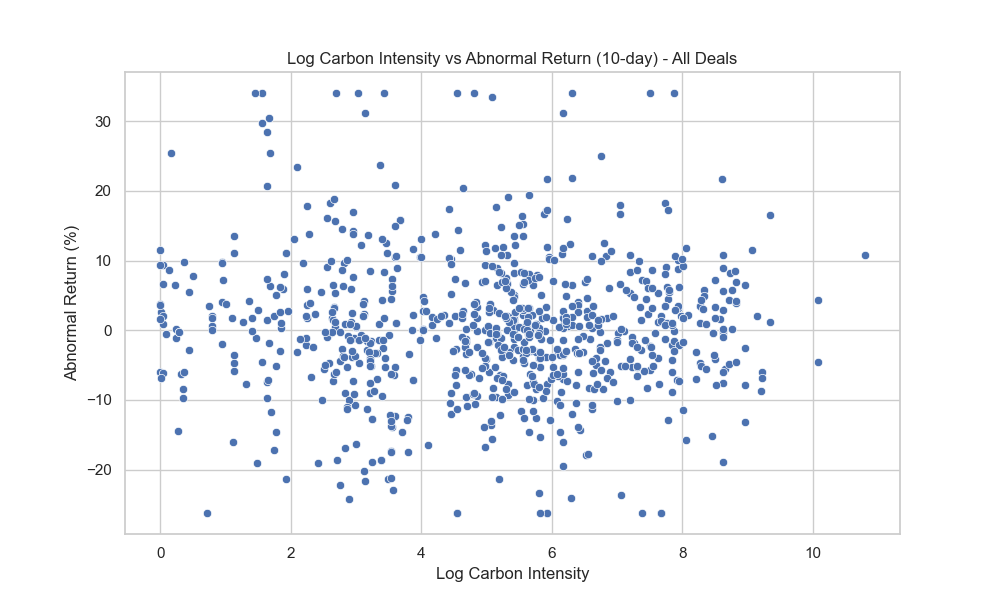
\includegraphics[width=\textwidth]{visualizations1/all_deals_10day_carbon_vs_ar.png}
        \caption{Log CI Vs AR regression}
        \label{fig:10day_ACIAR}
    \end{minipage}
\end{figure}

\begin{figure}[htbp]
\caption*{Any Acquirer - Green Targets 10 Day Results}
   \begin{minipage}{0.48\textwidth}
        \centering
        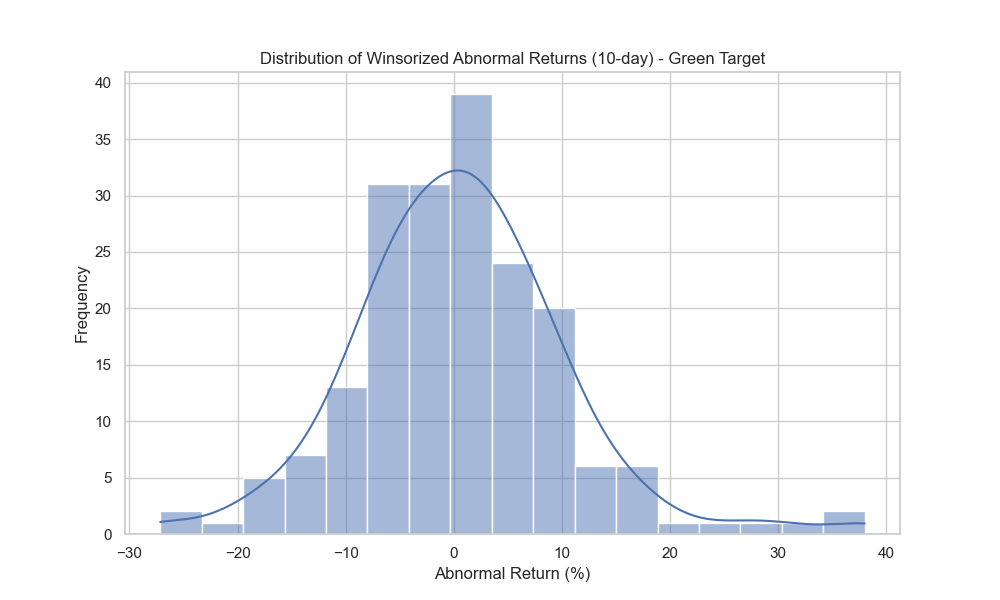
\includegraphics[width=\textwidth]{visualizations1/green_target_10day_ar_distribution.png}
        \caption{Abnormal Return Distribution}
        \label{fig:10day_GWARD}
    \end{minipage}
    \hfill
    \begin{minipage}{0.48\textwidth}
        \centering
        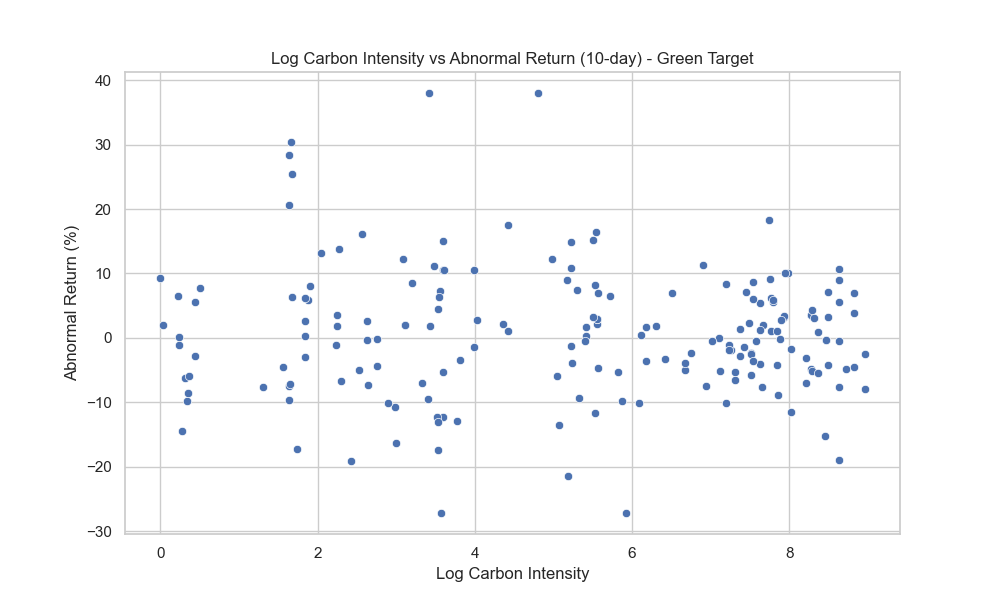
\includegraphics[width=\textwidth]{visualizations1/green_target_10day_carbon_vs_ar.png}
        \caption{Log CI Vs AR regression}
        \label{fig:10day_GCIAR}
    \end{minipage}
\end{figure}

\begin{figure}[htbp]
\caption*{Brown Acquirer - Green Targets 10 Day Results}
   \begin{minipage}{0.48\textwidth}
        \centering
        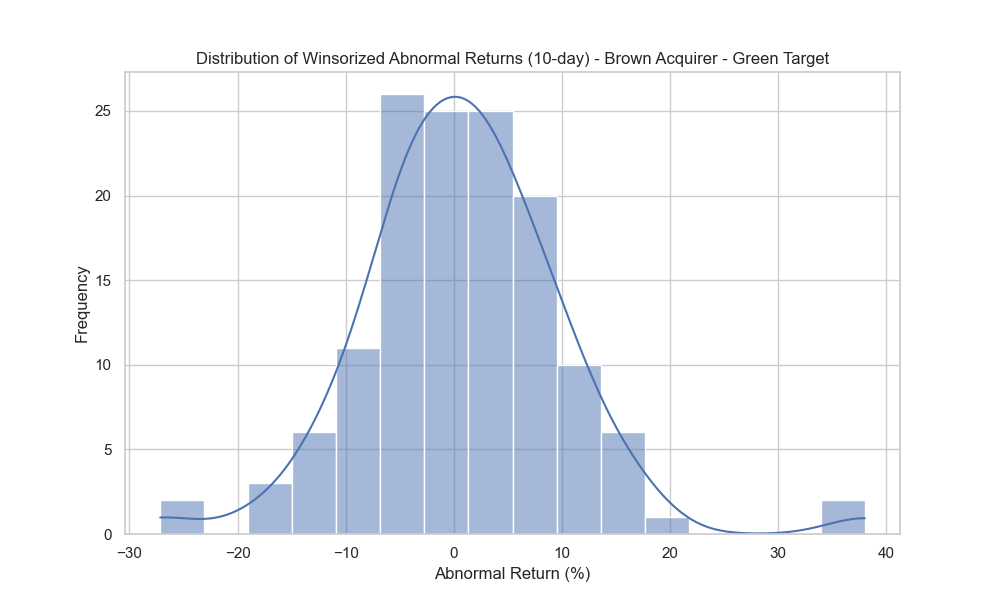
\includegraphics[width=\textwidth]{visualizations1/brown_acquirer_-_green_target_10day_ar_distribution.png}
        \caption{Abnormal Return Distribution}
        \label{fig:10day_BWARD}
    \end{minipage}
    \hfill
    \begin{minipage}{0.48\textwidth}
        \centering
        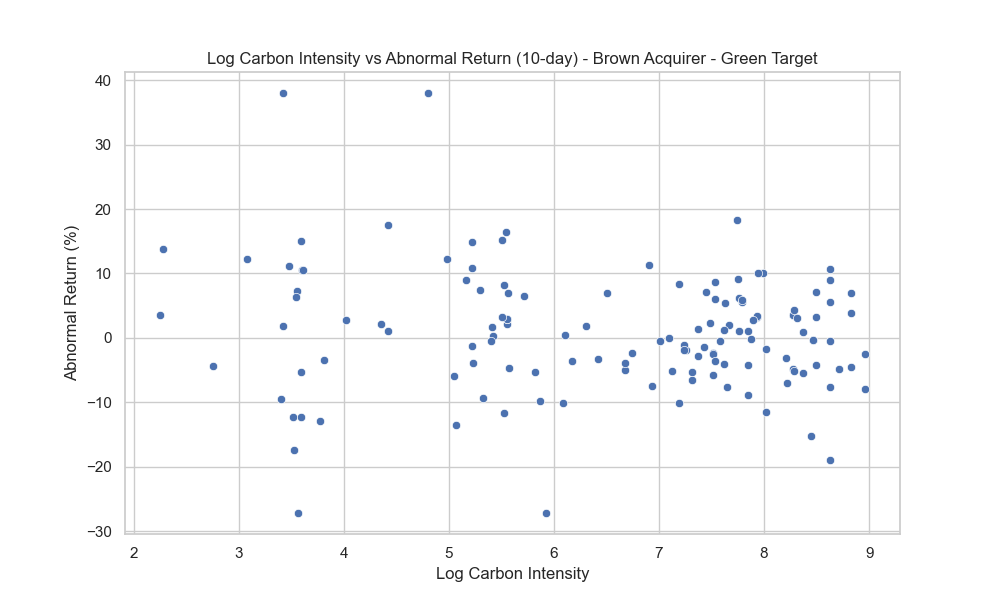
\includegraphics[width=\textwidth]{visualizations1/brown_acquirer_-_green_target_10day_carbon_vs_ar.png}
        \caption{Log CI Vs AR regression}
        \label{fig:10day_BCIAR}
    \end{minipage}
\end{figure}

\end{document}